\subsection{Practice 6}

Sketch the graph of the function $f(x) = x^3 - 3x^2 + 2$. \sol{}
\vspace{-0.6cm}
\begin{vwcol}[widths={0.5,0.5},justify=flush,rule=0pt,indent=1em]
    \begin{flalign*}
        f(0)                  & = 2                            & \\
        x^3 - 3x^2 + 2        & = 0                              \\
        (x - 1)(x^2 - 2x - 2) & = 0                              \\
        x = 1                 & \text{ or } x^2 - 2x - 2 = 0     \\
        x = 1                 & \text{ or } x = 1 \pm \sqrt{3}   \\
        f'(x)                 & = 3x^2 - 6x                    & \\
        f''(x)                & = 6x - 6                       & \\
        3x^2 - 6x             & = 0                            & \\
        x(x - 2)              & = 0                            & \\
        x = 0                 & \text{ or } x = 2              & \\
        f(0)                  & = 2                            & \\
        f(2)                  & = -2                           & \\
        f''(0)                & = -6 < 0                       & \\
        f''(2)                & = 6 > 0                        & \\
        6x - 6                & = 0                            & \\
        x                     & = 1                            & \\
        f(1)                  & = 0
    \end{flalign*}
    $x$-intercepts: $\left(1-\sqrt{3}, 0\right)$, $(1, 0)$, $\left(1+\sqrt{3}, 0\right)$

    \noindent $y$-intercept: $(0, 2)$

    \noindent Relative maximum: $(0, 2)$

    \noindent Relative minimum: $(2, -2)$

    \noindent Points of inflection: $(1, 0)$

    \noindent Convex up: $(-\infty, 1)$

    \noindent Convex down: $(1, \infty)$

    \pagebreak

    \vspace*{4cm}

    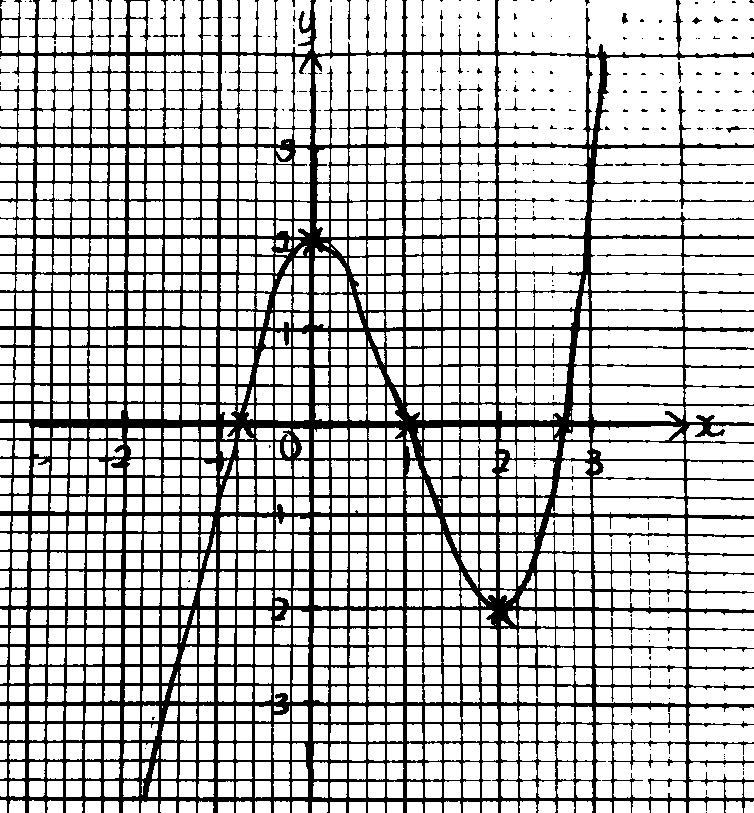
\includegraphics[scale=0.3]{assets/28-graph.jpeg}
\end{vwcol}